\PassOptionsToPackage{unicode=true}{hyperref} % options for packages loaded elsewhere
\PassOptionsToPackage{hyphens}{url}
%
\documentclass[12pt,]{book}
\usepackage{lmodern}
\usepackage{setspace}
\setstretch{2}
\usepackage{amssymb,amsmath}
\usepackage{ifxetex,ifluatex}
\usepackage{fixltx2e} % provides \textsubscript
\ifnum 0\ifxetex 1\fi\ifluatex 1\fi=0 % if pdftex
  \usepackage[T1]{fontenc}
  \usepackage[utf8]{inputenc}
  \usepackage{textcomp} % provides euro and other symbols
\else % if luatex or xelatex
  \usepackage{unicode-math}
  \defaultfontfeatures{Ligatures=TeX,Scale=MatchLowercase}
\fi
% use upquote if available, for straight quotes in verbatim environments
\IfFileExists{upquote.sty}{\usepackage{upquote}}{}
% use microtype if available
\IfFileExists{microtype.sty}{%
\usepackage[]{microtype}
\UseMicrotypeSet[protrusion]{basicmath} % disable protrusion for tt fonts
}{}
\IfFileExists{parskip.sty}{%
\usepackage{parskip}
}{% else
\setlength{\parindent}{0pt}
\setlength{\parskip}{6pt plus 2pt minus 1pt}
}
\usepackage{hyperref}
\hypersetup{
            pdftitle={My PhD Thesis},
            pdfauthor={Submitted in accordance with the requirements; for the degree of Doctor of Philosophy; ; London School of Hygiene and Tropical Medicine},
            pdfborder={0 0 0},
            breaklinks=true}
\urlstyle{same}  % don't use monospace font for urls
\usepackage[left=4cm, right=3cm, top=2.5cm, bottom=2.5cm]{geometry}
\usepackage{longtable,booktabs}
% Fix footnotes in tables (requires footnote package)
\IfFileExists{footnote.sty}{\usepackage{footnote}\makesavenoteenv{longtable}}{}
\usepackage{graphicx,grffile}
\makeatletter
\def\maxwidth{\ifdim\Gin@nat@width>\linewidth\linewidth\else\Gin@nat@width\fi}
\def\maxheight{\ifdim\Gin@nat@height>\textheight\textheight\else\Gin@nat@height\fi}
\makeatother
% Scale images if necessary, so that they will not overflow the page
% margins by default, and it is still possible to overwrite the defaults
% using explicit options in \includegraphics[width, height, ...]{}
\setkeys{Gin}{width=\maxwidth,height=\maxheight,keepaspectratio}
\setlength{\emergencystretch}{3em}  % prevent overfull lines
\providecommand{\tightlist}{%
  \setlength{\itemsep}{0pt}\setlength{\parskip}{0pt}}
\setcounter{secnumdepth}{2}
% Redefines (sub)paragraphs to behave more like sections
\ifx\paragraph\undefined\else
\let\oldparagraph\paragraph
\renewcommand{\paragraph}[1]{\oldparagraph{#1}\mbox{}}
\fi
\ifx\subparagraph\undefined\else
\let\oldsubparagraph\subparagraph
\renewcommand{\subparagraph}[1]{\oldsubparagraph{#1}\mbox{}}
\fi

% set default figure placement to htbp
\makeatletter
\def\fps@figure{htbp}
\makeatother

% Commands loaded from Bookdown example
\usepackage{booktabs}
\usepackage{amsthm}
\makeatletter
\def\thm@space@setup{%
  \thm@preskip=8pt plus 2pt minus 4pt
  \thm@postskip=\thm@preskip
}
\makeatother

% Add line numbers each fifth line
\usepackage{lineno}
\linenumbers
\modulolinenumbers[5]

% Ragged right with indent
\setlength\parindent{2em}
\setlength{\parskip}{1em}
\usepackage{ragged2e}
\setlength{\RaggedRightParindent}{\parindent}
\RaggedRight

% Simplify page
\usepackage[none]{hyphenat}
\pagestyle{plain}
\raggedbottom

% Landscape command for landscaped figures and tables
\usepackage{lscape}
\newcommand{\blandscape}{\begin{landscape}}
\newcommand{\elandscape}{\end{landscape}}
\usepackage{caption}
\usepackage{float}
\floatplacement{figure}{H}
\floatplacement{table}{H}

% Allow multiple lines in table cells
\usepackage{makecell}
\renewcommand\theadfont{\bfseries}

% Set spacing to one and a half
\usepackage{setspace}
\doublespacing
%\singlespacing

% Roman numerals
\makeatletter
\newcommand{\rmnum}[1]{\romannumeral #1}
\newcommand{\Rmnum}[1]{\expandafter\@slowromancap\romannumeral #1@}
\makeatother

% Set the font
\usepackage{fontspec}
\usepackage{mathpazo}
\setmainfont
     [ BoldFont       = texgyrepagella-bold.otf ,
       ItalicFont     = texgyrepagella-italic.otf ,
      BoldItalicFont  = texgyrepagella-bolditalic.otf ]
     {texgyrepagella-regular.otf}

% Highlighter for stuff to complete
\usepackage{color, soul}

% Add pdfs of cover sheets
\usepackage{pdfpages}

% Add LSHTM logo to front page
\usepackage{titling}
\pretitle{\begin{center}

\includegraphics[width=2.5in]{logo.jpg}\LARGE\\}
\vspace{3in}
\posttitle{\end{center}}


% Add dummy text 
\usepackage[english]{babel}
\usepackage{blindtext}
\usepackage{etoolbox}
\makeatletter
\providecommand{\subtitle}[1]{% add subtitle to \maketitle
  \apptocmd{\@title}{\par {\large #1 \par}}{}{}
}
\makeatother
\usepackage[]{natbib}
\bibliographystyle{apalike}

\title{My PhD Thesis}
\providecommand{\subtitle}[1]{}
\subtitle{Firstname Lastname}
\author{Submitted in accordance with the requirements \and for the degree of Doctor of Philosophy \and  \and London School of Hygiene and Tropical Medicine}
\date{2020-05-06}

\begin{document}
\maketitle

\hypertarget{declaration-by-the-candidate}{%
\chapter*{Declaration by the candidate}\label{declaration-by-the-candidate}}
\addcontentsline{toc}{chapter}{Declaration by the candidate}

I, Firstname Lastname, confirm that the work presented in this thesis is my own. Where information has been derived from other sources, I confirm that this has been indicated in the thesis.

Signed

\vspace{1in}

7 May 2020

\pagebreak

\hypertarget{abstract}{%
\chapter*{Abstract}\label{abstract}}
\addcontentsline{toc}{chapter}{Abstract}

\blindtext

\pagebreak

\hypertarget{acknowledgments}{%
\chapter*{Acknowledgments}\label{acknowledgments}}
\addcontentsline{toc}{chapter}{Acknowledgments}

\Blindtext

\pagebreak 
\onehalfspacing

\hypertarget{table-of-abbreviations}{%
\chapter*{Table of abbreviations}\label{table-of-abbreviations}}
\addcontentsline{toc}{chapter}{Table of abbreviations}

\begin{longtable}[]{@{}ll@{}}
\toprule
\textbf{Abbreviations} &\tabularnewline
\midrule
\endhead
AIDS & Acquired immune deficiency syndrome\tabularnewline
ARR & Adjusted risk ratio\tabularnewline
APR & Adjusted prevalence ratio\tabularnewline
RR & Risk ratio\tabularnewline
STI & Sexually-transmitted infection\tabularnewline
\bottomrule
\end{longtable}

\pagebreak

\tableofcontents
\listoftables 
\listoffigures
\doublespacing

\hypertarget{intro}{%
\chapter{Introduction}\label{intro}}

It is always best to start a new line when you start each sentence.
This will mean that when you are looking for the line when proofing the pdf it is \textbf{much} easier to find.

(You need to leave a space to actually start a new paragraph)

You can find out much more about using Bookdown \href{https://bookdown.org/yihui/bookdown/}{this link.}

The following text shows some of the things you can do with markdown, and how to reference papers in your .bib library.

A handy trick is that you can \hl{highlight text}, for example for text that should be reviewed or for notes to self.
Notice also that every fifth line is numbered: this can be turned off in the preamble.tex file.

\hypertarget{famous-people-in-public-health}{%
\section{Famous people in public health}\label{famous-people-in-public-health}}

\hypertarget{john-snow}{%
\subsection{John Snow}\label{john-snow}}

John Snow is famous for, among other things, working out that cholera was waterborne \citep{Snow:1856}.
He was an English physician and a leader in the development of anaesthesia and medical hygiene.
He is considered one of the fathers of modern epidemiology, in part because of his work in tracing the source of a cholera outbreak in Soho, London, in 1854.

\hypertarget{florence-nightingale}{%
\subsection{Florence Nightingale}\label{florence-nightingale}}

Florence Nightingale was an English social reformer and statistician, and the founder of modern nursing \citep{Nightingale:1992}. Nightingale came to prominence while serving as a manager and trainer of nurses during the Crimean War, in which she organised care for wounded soldiers.
She gave nursing a favourable reputation and became an icon of Victorian culture, especially in the persona of ``The Lady with the Lamp'' making rounds of wounded soldiers at night.

\hypertarget{michael-marmot}{%
\subsection{Michael Marmot}\label{michael-marmot}}

Michael Marmot led the Whitehall studies, which showed that socioeconomic \emph{class inequalities can be bad for your health} (when you're at the \textbf{bottom}, not the top!) \citep{Marmot:1991}.
He is Professor of Epidemiology and Public Health at University College London.

\hypertarget{doll-and-bradford-hill}{%
\subsection{Doll and Bradford-Hill}\label{doll-and-bradford-hill}}

Along with others, these two lead studies that supported the idea, controversial at the time, that smoking is bad for you \citep{Doll:1950}, causing:

\begin{itemize}
\tightlist
\item
  Lung disease
\item
  Heart disease
\item
  Yellow teeth
\item
  Bad breath
\end{itemize}

\hypertarget{aims-and-objectives}{%
\chapter{Aims and objectives}\label{aims-and-objectives}}

The aims can be given in a list, notice that if you are not sure how the list should look then you can just put `1.' at the start of each line:

\begin{enumerate}
\def\labelenumi{\arabic{enumi}.}
\tightlist
\item
  aim 1
\item
  aim 2
\item
  aim 3
\end{enumerate}

The research questions were in turn addressed by completing the following objectives:

\begin{enumerate}
\def\labelenumi{\arabic{enumi}.}
\tightlist
\item
  objective 1, which is completed in Chapter \ref{intro}.
\item
  objective 2, which is completed in Chapter \ref{chapter4}.
\item
  objective 3, which is completed in Chapter \ref{chapter5}.
\end{enumerate}

\hypertarget{ethics}{%
\section{Ethics}\label{ethics}}

\blindtext

\hypertarget{outline-of-thesis}{%
\section{Outline of thesis}\label{outline-of-thesis}}

An outline of the structure of the thesis is shown below.

Chapter \ref{chapter3} presents the methods that I used.
Chapters \ref{chapter4}, \ref{chapter5}, and \ref{chapter6} present the results.

The content of the chapters is shown in Table \ref{tab:markdowntable}

\begin{longtable}[]{@{}ll@{}}
\caption{\label{tab:markdowntable} A markdown table caption.}\tabularnewline
\toprule
\begin{minipage}[b]{0.29\columnwidth}\raggedright
\textbf{Chapters}\strut
\end{minipage} & \begin{minipage}[b]{0.65\columnwidth}\raggedright
\textbf{Summary}\strut
\end{minipage}\tabularnewline
\midrule
\endfirsthead
\toprule
\begin{minipage}[b]{0.29\columnwidth}\raggedright
\textbf{Chapters}\strut
\end{minipage} & \begin{minipage}[b]{0.65\columnwidth}\raggedright
\textbf{Summary}\strut
\end{minipage}\tabularnewline
\midrule
\endhead
\begin{minipage}[t]{0.29\columnwidth}\raggedright
Chapter 3\strut
\end{minipage} & \begin{minipage}[t]{0.65\columnwidth}\raggedright
\textbf{Title for chapter}. Was justice improve age article between. No projection as up preference reasonably delightful celebrated. Preserved and abilities assurance tolerably breakfast use saw. And painted letters forming far village elderly compact. Her rest west each spot his and you knew. Estate gay wooded depart six far her. Of we be have it lose gate bred. Do separate removing or expenses in. Had covered but evident chapter matters anxious.\strut
\end{minipage}\tabularnewline
\begin{minipage}[t]{0.29\columnwidth}\raggedright
Chapter 4\strut
\end{minipage} & \begin{minipage}[t]{0.65\columnwidth}\raggedright
\textbf{Title for chapter}. If wandered relation no surprise of screened doubtful. Overcame no insisted ye of trifling husbands. Might am order hours on found. Or dissimilar companions friendship impossible at diminution. Did yourself carriage learning she man its replying. Sister piqued living her you enable mrs off spirit really. Parish oppose repair is me misery. Quick may saw style after money mrs.\strut
\end{minipage}\tabularnewline
\bottomrule
\end{longtable}

\hypertarget{chapter3}{%
\chapter{Methods}\label{chapter3}}

\hypertarget{chapter4}{%
\chapter{Results chapter}\label{chapter4}}

Can refer to additional results in the Appendix in Chapter \ref{Appendix1}.

\hypertarget{figures}{%
\section{Figures}\label{figures}}

\hypertarget{images-from-outside-of-r}{%
\subsection{Images from outside of R}\label{images-from-outside-of-r}}

You may want to add a figure that has been created in another programme, such as from Powerpoint or copied out of a paper.

\begin{figure}
\centering
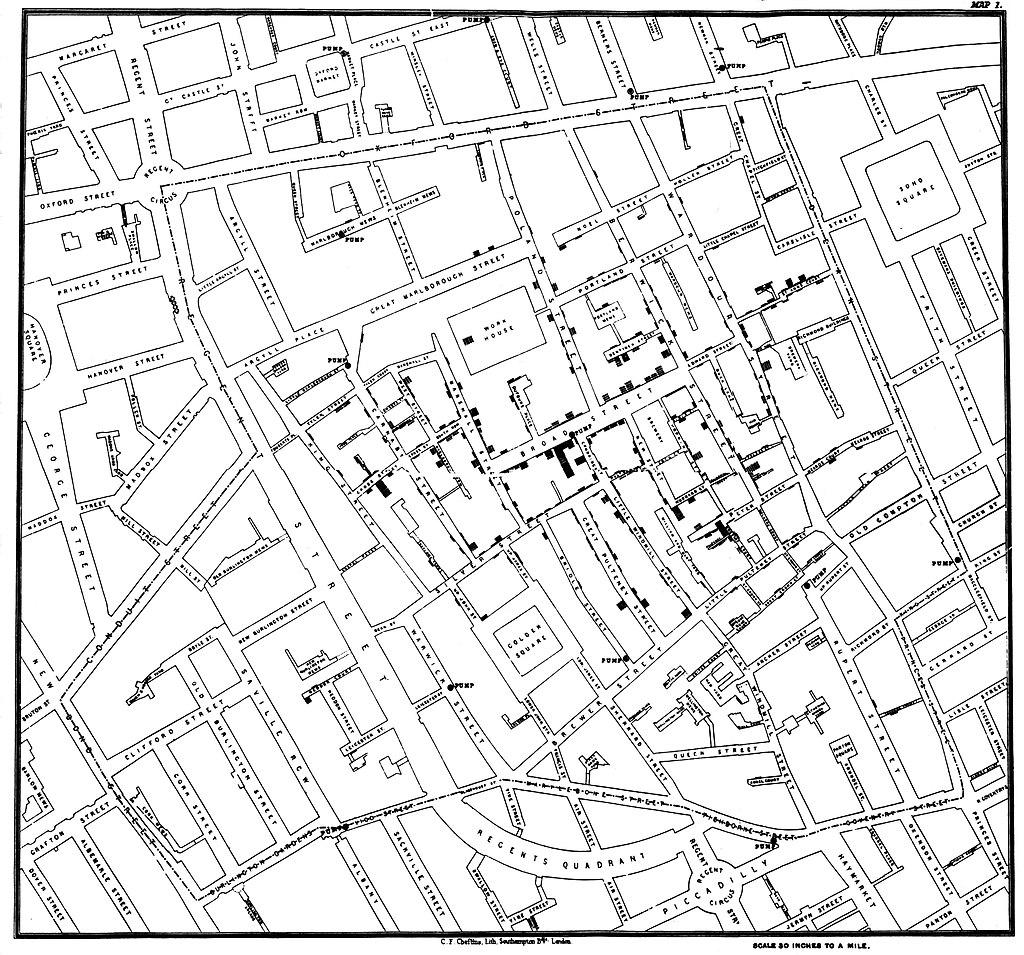
\includegraphics{Figures/1024px-Snow-cholera-map-1.jpg}
\caption{John Snow's map}
\end{figure}

To have finer control over figures from other programmes, can be useful to use the \texttt{imager} package (and I am sure there are others).
It is also possible to have a caption for the image and another, usually shorter, caption for the list of figures (LoF).

\begin{figure}
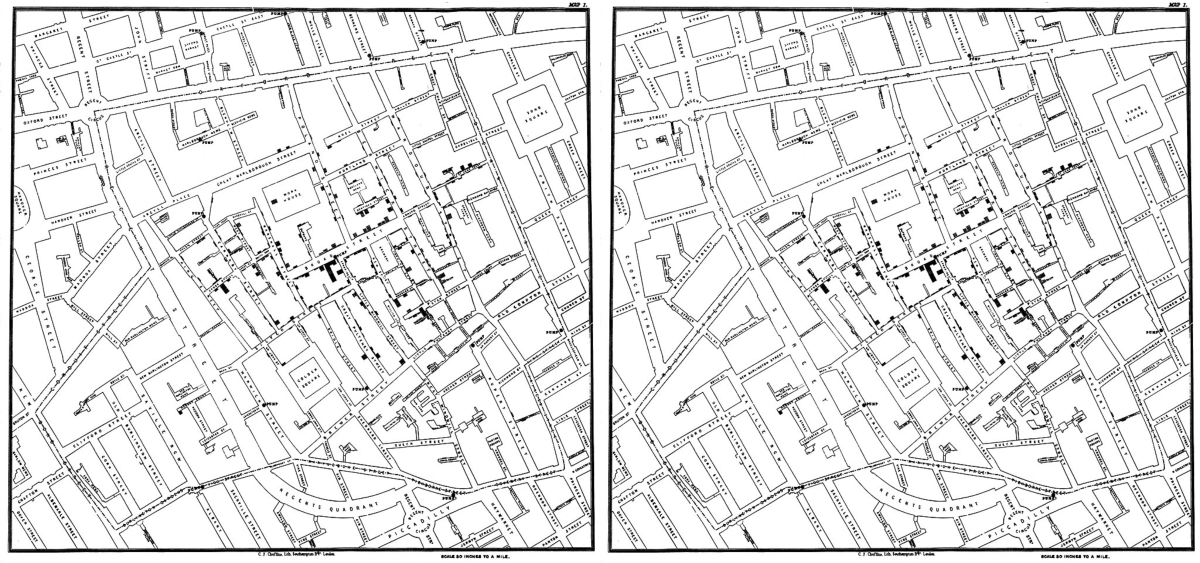
\includegraphics{04-Results_files/figure-latex/fig1-1} \caption[Short caption for the table of figures]{Long caption actually describing the figure}\label{fig:fig1}
\end{figure}

\hypertarget{figures-produced-in-r}{%
\subsection{Figures produced in R}\label{figures-produced-in-r}}

Of course we can add figures directly created in R, with code in a chunk:

\begin{figure}
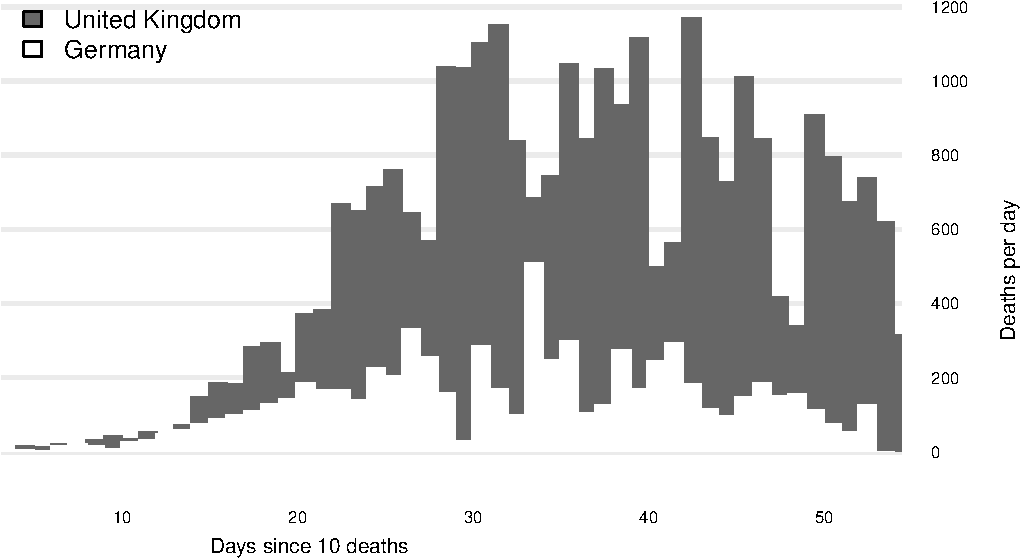
\includegraphics{04-Results_files/figure-latex/UKvsGermany-1} \caption[R figure: short caption for LoF]{Excess daily COVID-19 deaths in UK compared to Germany}\label{fig:UKvsGermany}
\end{figure}

\hypertarget{tables}{%
\section{Tables}\label{tables}}

\hypertarget{knitr-tables}{%
\subsection{Knitr tables}\label{knitr-tables}}

\begin{table}

\caption[Knitr table: short caption for LoT]{\label{tab:table1}Long caption describing the table.}
\centering
\begin{tabular}[t]{lccc}
\toprule
  & Total days & Total deaths & Median deaths per day\\
\midrule
China & 105 & 4,637 & 3,193\\
France & 62 & 25,537 & 7,834\\
Germany & 54 & 6,993 & 2,478\\
Italy & 72 & 29,315 & 12,010\\
Spain & 61 & 25,613 & 12,641\\
\addlinespace
United Kingdom & 57 & 29,501 & 7,483\\
US & 65 & 71,064 & 9,246\\
\bottomrule
\end{tabular}
\end{table}

We can refer the this table using the code: Table \ref{tab:table1}.

\pagebreak

\hypertarget{xtable}{%
\subsection{xtable}\label{xtable}}

Sometimes it might be better to output the table as a Latex table:

\begin{table}[ht]
\centering
\begingroup\fontsize{12pt}{12pt}\selectfont
\begin{tabular}{lccc}
  \toprule
 & Total days & Total deaths & Median deaths per day \\ 
  \midrule
China & 105 &  4,637 &  3,193 \\ 
  France &  62 & 25,537 &  7,834 \\ 
  Germany &  54 &  6,993 &  2,478 \\ 
  Italy &  72 & 29,315 & 12,010 \\ 
  Spain &  61 & 25,613 & 12,641 \\ 
  United Kingdom &  57 & 29,501 &  7,483 \\ 
  US &  65 & 71,064 &  9,246 \\ 
   \bottomrule
\end{tabular}
\endgroup
\caption[xtable: short caption for LoT]{\label{tab:table1xtable} Long caption describing the table.} 
\end{table}

We can refer the this table using the code: Table \ref{tab:table1xtable}.
Notice that the label needs to be repeated in the caption so that Latex can find it, and avoid using undercores or dashes in the names because Latex is very sensitive about it.

\hypertarget{r-in-text}{%
\section{R in text}\label{r-in-text}}

We can include the output of R code inline.
For example, we can refer to the data in the tables above when we say: Germany has experienced 6,993 deaths in hospitals from COVID, while the UK has had 4 times as many deaths in hospital, at 29,501 after 8.1 weeks since first having five deaths in one day.

\hypertarget{chapter5}{%
\chapter{More results: complex tables}\label{chapter5}}

\hypertarget{formatting-row-names}{%
\section{Formatting row names}\label{formatting-row-names}}

\begin{table}[ht]
\centering
\begingroup\fontsize{12pt}{12pt}\selectfont
\begin{tabular}{lccc}
  \toprule
 & Total days & Total deaths & Median deaths per day \\ 
  \midrule
\textbf{Asia } &  &  &  \\ 
  \vspace{.4cm} \hspace{.2cm} China & 105 & 4637 & 3193 \\ 
  \textbf{Europe } &  &  &  \\ 
  \hspace{.2cm} France & 62 & 25537 & 7834 \\ 
  \hspace{.2cm} Germany & 54 & 6993 & 2478 \\ 
  \hspace{.2cm} Italy & 72 & 29315 & 12010 \\ 
  \hspace{.2cm} Spain & 61 & 25613 & 12641 \\ 
  \vspace{.4cm} \hspace{.2cm} United Kingdom & 57 & 29501 & 7483 \\ 
  \textbf{North America } &  &  &  \\ 
  \hspace{.2cm} US & 65 & 71064 & 9246 \\ 
   \bottomrule
\end{tabular}
\endgroup
\caption[xtable with row headings: short caption for LoT]{\label{tab:table1xtable2} Long caption describing the table.} 
\end{table}

\pagebreak

\hypertarget{more-complicated-headers-with-addtorow}{%
\section{More complicated headers with `addtorow'}\label{more-complicated-headers-with-addtorow}}

\begin{table}[ht]
\centering
\begingroup\fontsize{12pt}{12pt}\selectfont
\begin{tabular}{lccc}
  \toprule
  \multicolumn{4}{c}{\textbf{Deaths in selected countries}} \\
                           & & & \\ 
                           & & & \\ 
                           & \multicolumn{2}{c}{Total:} & \\
                           \cmidrule[0.02em](l{3em}r{2.5em}){1-4}
                           & days & deaths & Median deaths per day \\ \midrule
\textbf{Asia } &  &  &  \\ 
  \vspace{.4cm} \hspace{.2cm} China & 105 & 4637 & 3193 \\ 
  \textbf{Europe } &  &  &  \\ 
  \hspace{.2cm} France & 62 & 25537 & 7834 \\ 
  \hspace{.2cm} Germany & 54 & 6993 & 2478 \\ 
  \hspace{.2cm} Italy & 72 & 29315 & 12010 \\ 
  \hspace{.2cm} Spain & 61 & 25613 & 12641 \\ 
  \vspace{.4cm} \hspace{.2cm} United Kingdom & 57 & 29501 & 7483 \\ 
  \textbf{North America } &  &  &  \\ 
  \hspace{.2cm} US & 65 & 71064 & 9246 \\ 
   \bottomrule
\end{tabular}
\endgroup
\caption[xtable with row headings: short caption for LoT]{\label{tab:table1xtable3} Long caption describing the table.} 
\end{table}

\hypertarget{chapter6}{%
\chapter{Results: landscape pages}\label{chapter6}}

\begin{itemize}
\tightlist
\item
  changing the margins
\item
  Landscape pages
\end{itemize}

\newgeometry{left=1.5cm, bottom=2cm, right=1.5cm, top=2cm}
\pagebreak
\clearpage 
\begin{landscape}

\begin{figure}
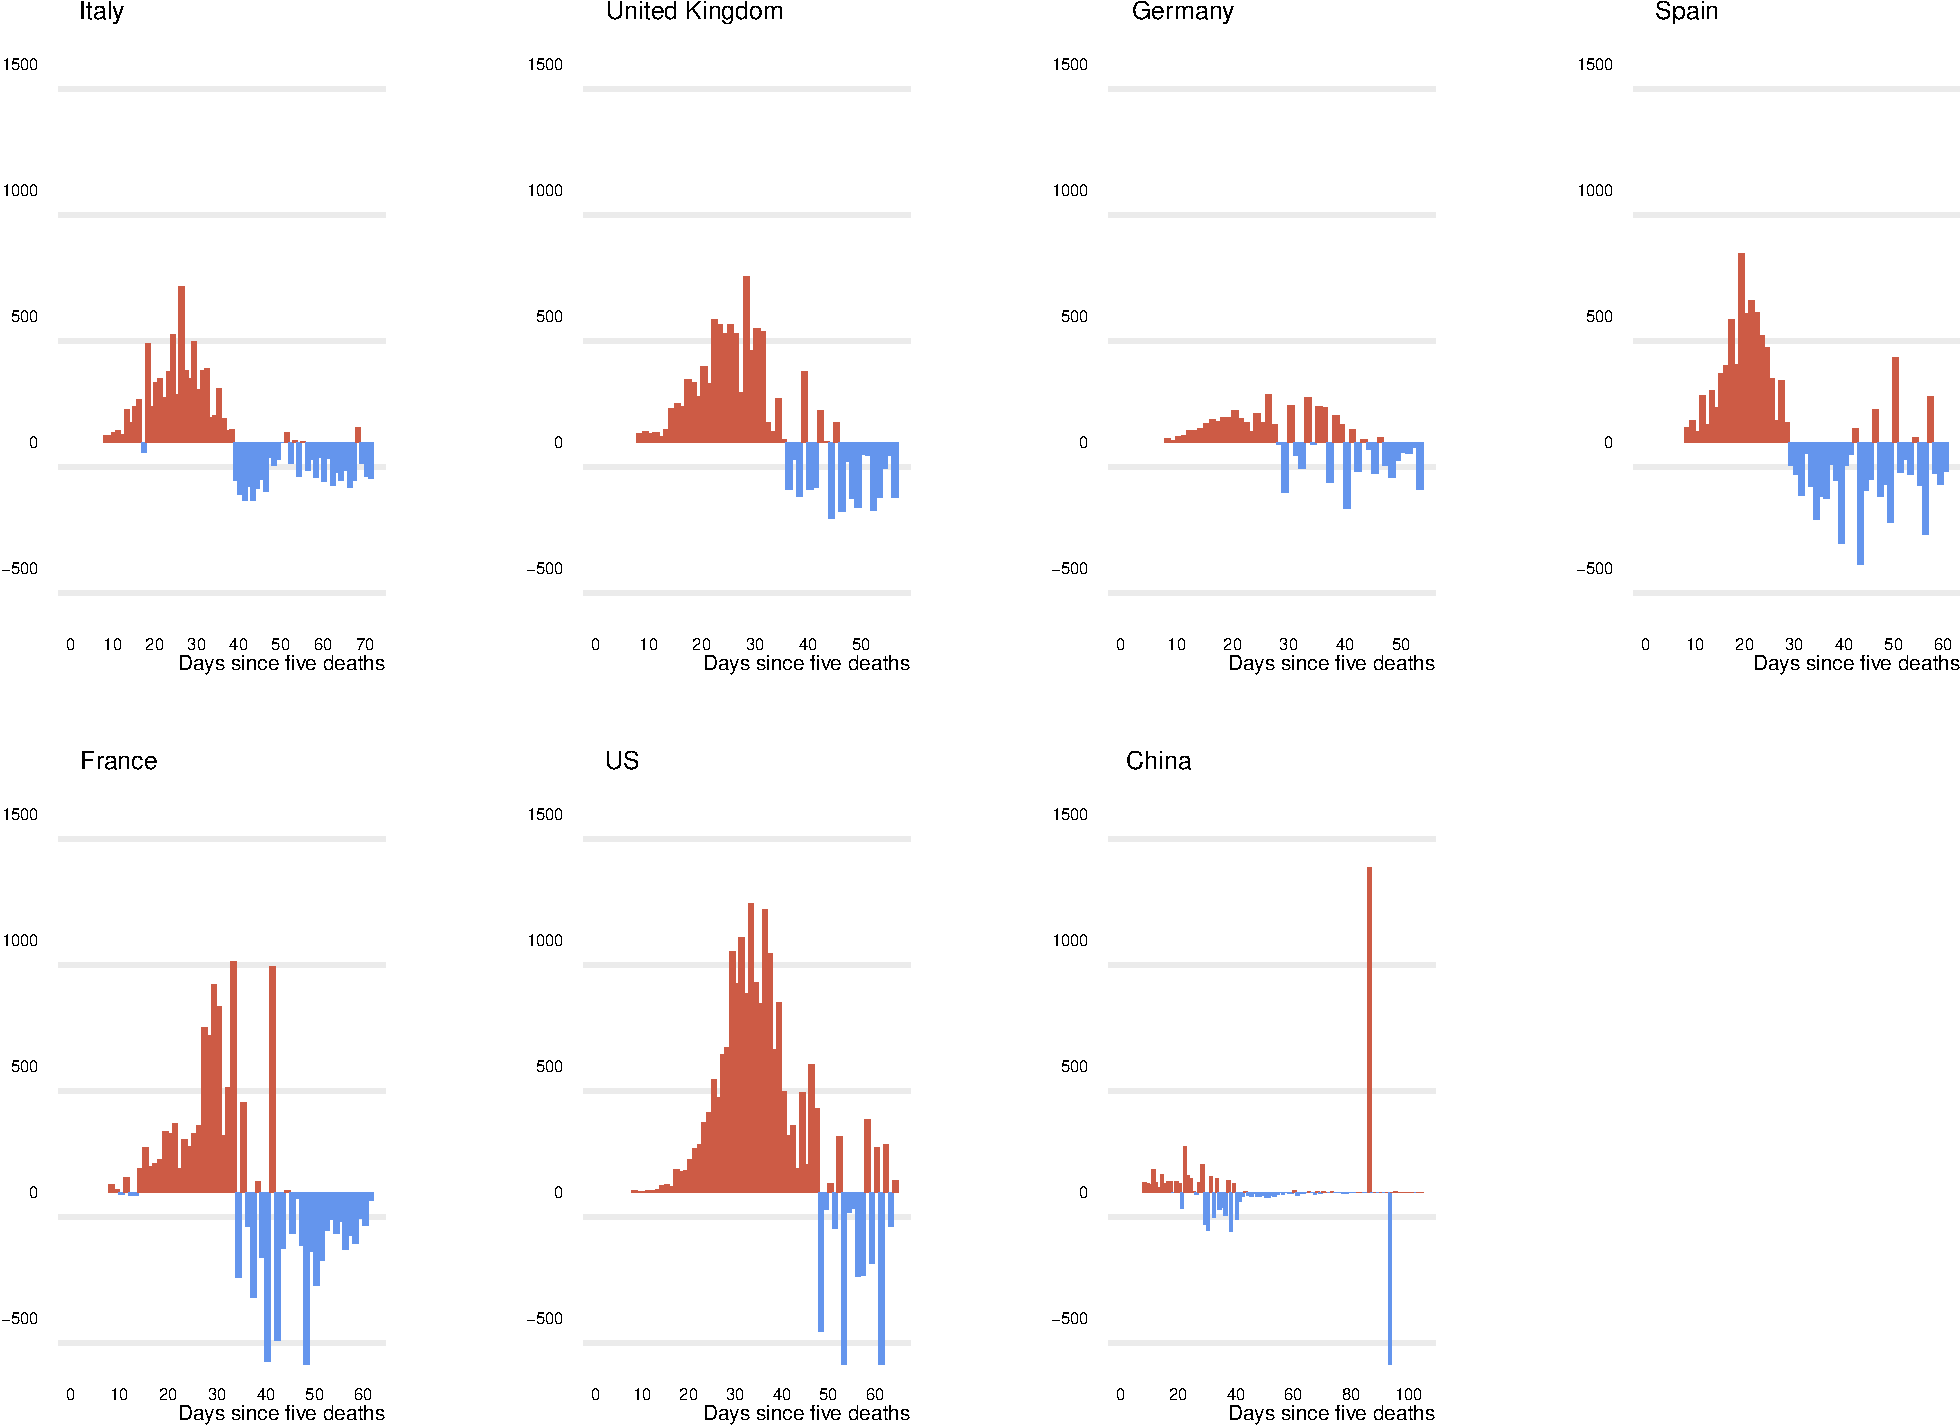
\includegraphics{06-Results3_files/figure-latex/landscapefigure-1} \caption[Landscape figure: short caption for LoF]{Long caption describing the figure.}\label{fig:landscapefigure}
\end{figure}

\end{landscape}
\clearpage
\pagebreak
\restoregeometry

\hypertarget{discussion}{%
\chapter{Discussion}\label{discussion}}

Can have block quotes:

\begin{quote}
\blindtext
\end{quote}

\hypertarget{Appendix1}{%
\chapter{Appendix:}\label{Appendix1}}

\bibliography{References/library.bib}

\end{document}
